%===================================================================================%
%          Présentation du système modélisé (les marchands et les clients)          %
%===================================================================================%


Le logiciel modélise une interaction entre des acheteurs et des marchands dans une rue commerçante.

\subsection{Présentation générale}

Des clients (\texttt{Buyer}) se baladent et veulent acheter des articles à des marchands (\texttt{Seller}).

\vspace{1cm}
\begin{figure}[h]
    \centering
    \fbox{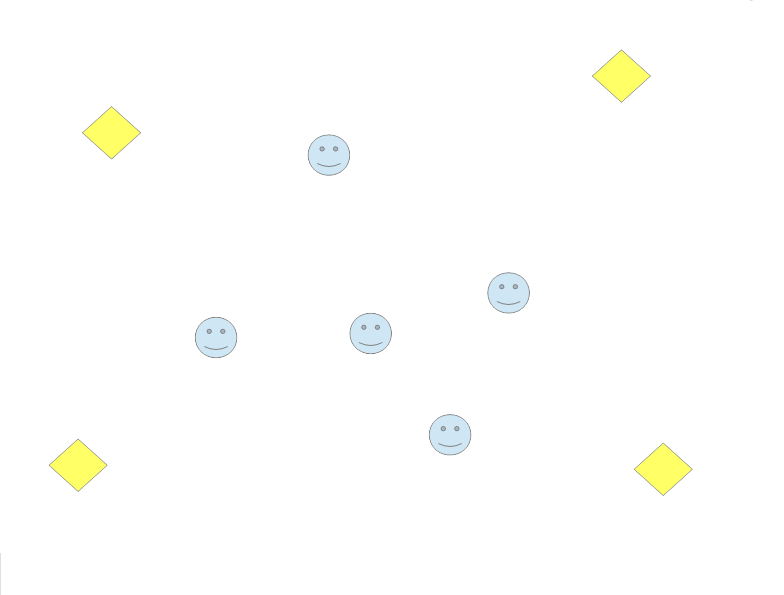
\includegraphics[height=200pt]{images/schemas/systeme.png}}
    \caption{\label{systeme}Description}
\end{figure}

L'interaction sociale se fait entre clients afin d'échanger la connaissance des prix qu'ils ont obtenue auprès des marchands, de manière à aller vers le marchand le moins onéreux.


\subsection{Description des objets}

\begin{itemize}
\item
	\texttt{Buyer} :\\
	Un acheteur est caractérisé par sa position, sa direction
	et la connaissance d'un marchand comme étant le moins cher.\\
	Il possède des méthodes pour se déplacer et obtenir une information auprès d'un autre acheteur ou d'un client.
	
\item
	\texttt{Seller}:\\
	Un vendeur est caractérisé par sa position et son prix.\\
	Il possède une méthode lui permettant de donner son prix.
	
\end{itemize}


\subsection{Déroulement de l'algorithme}

Au départ, les clients sont placés aléatoirement sur la grille, les marchands ayant des positions fixes. Aucune connaissance n'est donnée sur le prix et c'est aux clients d'aller chercher l'information.

Un client donné se dirige vers un marchand pris au hasard. Arrivé à ce marchand, il choisit d'acheter ou non en fonction de sa connaissance des prix : s'il en connaît un moins cher ailleurs, il y va ; sinon, il achète.
S'il croise un autre client, ils échangent leur connaissance du marchand meilleur marché et ne gardent l'information acquise que si elle est plus intéressante que la leur.
